\noindent\textbf{Atores do Sistema:}
\begin{itemize}[itemsep=0.6em, topsep=0.3em, parsep=0pt]
    \item \textbf{Usuário (Cliente)}: acessa o sistema para realizar cadastro/login, consultar informações, criar/editar solicitações e acompanhar status.
    \item \textbf{Administrador}: gerencia cadastros, permissões, configurações gerais e monitora registros/relatórios.
    \item \textbf{Operador/Atendente}: valida dados enviados pelos usuários, aprova/reprova solicitações e atualiza status operacionais.
    \item \textbf{Sistema Externo (API/Integrações)}: provê/autentica dados de serviços de terceiros (ex.: pagamento, mapas, notificações).
\end{itemize}

\vspace{0.9\baselineskip}

\noindent\textbf{Casos de Uso do Sistema:}
\begin{itemize}[itemsep=0.6em, topsep=0.3em, parsep=0pt]
    \item \textbf{Autenticar Usuário}: realizar cadastro, login e recuperação de senha.
    \item \textbf{Gerenciar Perfis}: editar dados pessoais, preferências e documentos.
    \item \textbf{Registrar Solicitação}: criar, editar e cancelar solicitações (com validações e anexos).
    \item \textbf{Acompanhar Status}: visualizar andamento, receber notificações e histórico.
    \item \textbf{Gerir Operações (Backoffice)}: triagem, aprovação/reprovação e ajustes operacionais.
    \item \textbf{Relatórios e Auditoria}: visualizar métricas, exportar dados e rastrear logs.
    \item \textbf{Integrações}: consultar/enviar dados para APIs externas (pagamentos, geolocalização, e-mail/SMS).
\end{itemize}

\begin{figure}[H]
\centering
\caption{Diagrama de caso de uso}
\label{fig:diagrama-caso-uso}
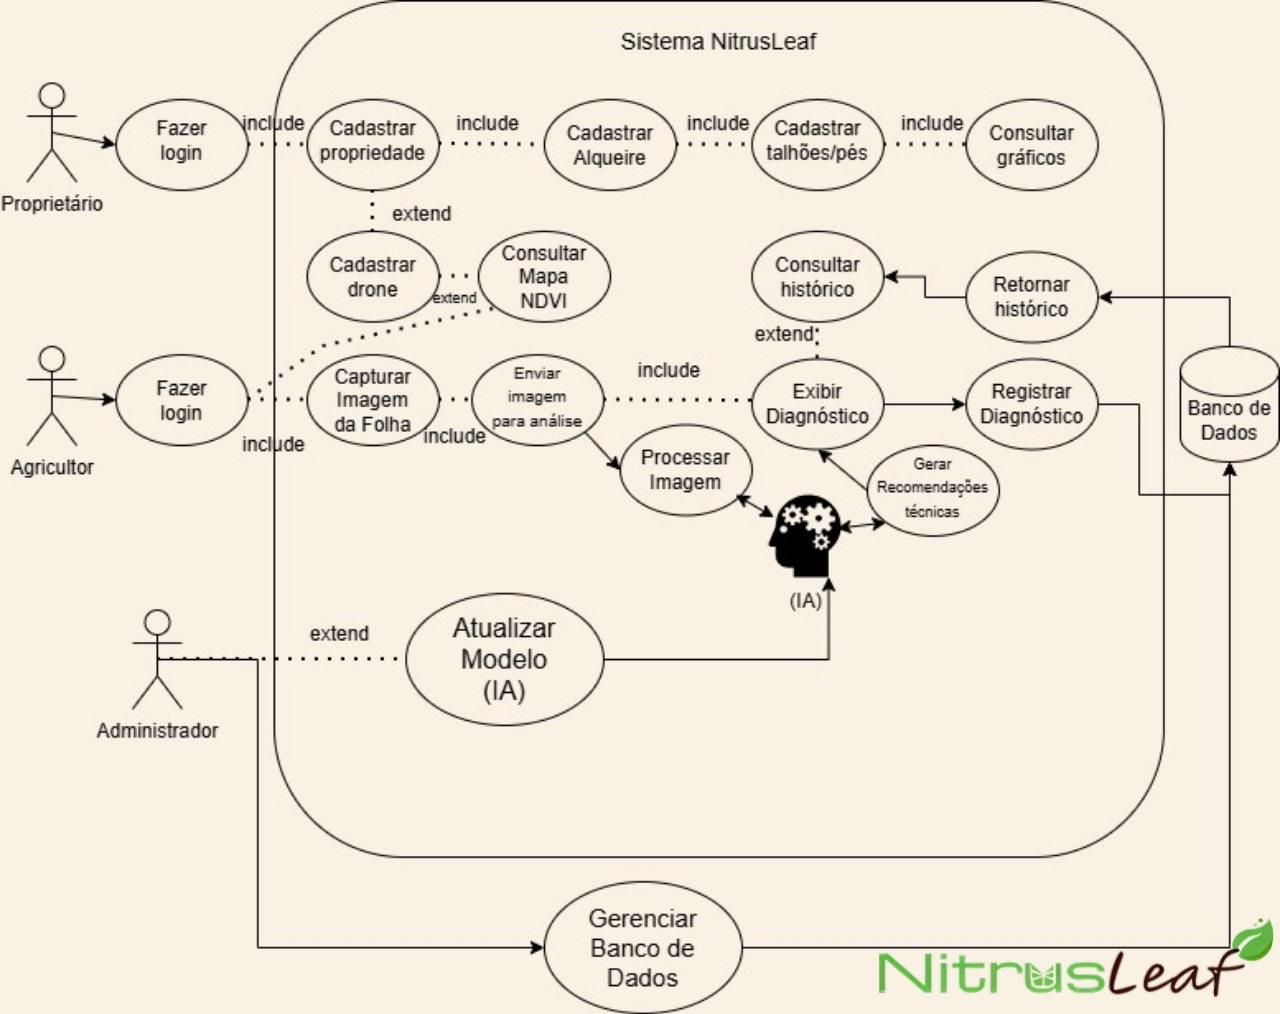
\includegraphics[width=0.8\textwidth]{Images/DiagramaCasosDeUso.jpg}
\SourceOrNote{Equipe 21 - Vitalliz (2025)}
\end{figure}

O diagrama acima ilustra as principais interações entre os usuários e o sistema,
evidenciando os processos relacionados ao monitoramento de deficiências nutricionais
em plantações de mexerica com o apoio de tecnologia de drones.
\medskip